\iftestbuild % TEST-ONLY-BEGIN
\setcounter{section}{5}\setcounter{theorem}{81}
\fi % TEST-ONLY-END
% Source: book pp. 280--296 (PDF 294--310); no solutions.
% \axeqno: see 7C.tex
\DeclareRobustCommand\axeqno{\refstepcounter{theorem}\tag*{\thetheorem}}
% the light blue of Axler's ellipsoid and box figures
\providecolor{axfigblue}{RGB}{166,212,255}
\section{Consequences of Singular Value Decomposition}

\subsection{Norms of Linear Maps}

The singular value decomposition leads to the following upper bound for
$\norm{Tv}$.

\begin{result}[Upper bound for $\norm{Tv}$]\label{ax:7.82}
Suppose $T\in\Lin(V,W)$. Let $s_1$ be the largest singular value of $T$. Then
\[ \norm{Tv}\le s_1\norm{v} \]
for all $v\in V$.
\end{result}

\begin{proof}
\marginnote[6mm]{For a lower bound on $\norm{Tv}$, look at Exercise~14 in
Section~7E.}%
Let $s_1,\dots,s_m$ denote the positive singular values of $T$, and let
$e_1,\dots,e_m$ be an orthonormal list in $V$ and $f_1,\dots,f_m$ be an
orthonormal list in $W$ that provide a singular value decomposition of $T$.
Thus
\[ Tv = s_1\ip{v}{e_1}f_1+\cdots+s_m\ip{v}{e_m}f_m \axeqno\label{ax:7.83} \]
for all $v\in V$. Hence if $v\in V$ then
\begin{align*}
\norm{Tv}^2 &= s_1^2\abs{\ip{v}{e_1}}^2+\cdots+s_m^2\abs{\ip{v}{e_m}}^2\\
  &\le s_1^2(\abs{\ip{v}{e_1}}^2+\cdots+\abs{\ip{v}{e_m}}^2)\\
  &\le s_1^2\norm{v}^2,
\end{align*}
where the last inequality follows from Bessel's inequality (\ref{ax:6.26}).
Taking square roots of both sides of the inequality above shows that
$\norm{Tv}\le s_1\norm{v}$, as desired.
\end{proof}

Suppose $T\in\Lin(V,W)$ and $s_1$ is the largest singular value of $T$. The
result above shows that
\[ \norm{Tv}\le s_1 \text{ for all } v\in V \text{ with } \norm{v}\le1.
   \axeqno\label{ax:7.84} \]
Taking $v=e_1$ in \ref{ax:7.83} shows that $Te_1=s_1f_1$. Because
$\norm{f_1}=1$, this implies that $\norm{Te_1}=s_1$. Thus because
$\norm{e_1}=1$, the inequality in \ref{ax:7.84} leads to the equation
\[ \max\{\norm{Tv} : v\in V \text{ and } \norm{v}\le1\} = s_1.
   \axeqno\label{ax:7.85} \]

The equation above is the motivation for the following definition, which
defines the norm of $T$ to be the left side of the equation above without
needing to refer to singular values or the singular value decomposition.

\begin{definition}[Norm of a linear map, $\norm{\cdot}$]\label{ax:7.86}
Suppose $T\in\Lin(V,W)$. Then the \emph{norm} of $T$, denoted by $\norm{T}$, is
defined by
\[ \norm{T} = \max\{\norm{Tv} : v\in V \text{ and } \norm{v}\le1\}. \]
\end{definition}

In general, the maximum of an infinite set of nonnegative numbers need not
exist. However, the discussion before \ref{ax:7.86} shows that the maximum in
the definition of the norm of a linear map $T$ from $V$ to $W$ does indeed
exist (and equals the largest singular value of $T$).

We now have two different uses of the word \emph{norm} and the notation
$\norm{\cdot}$. Our first use of this notation was in connection with an inner
product on $V$, when we defined $\norm{v}=\sqrt{\ip{v}{v}}$ for each $v\in V$.
Our second use of the norm notation and terminology is with the definition we
just made of $\norm{T}$ for $T\in\Lin(V,W)$. The norm $\norm{T}$ for
$T\in\Lin(V,W)$ does not usually come from taking an inner product of $T$ with
itself (see Exercise~21). You should be able to tell from the context and from
the symbols used which meaning of the norm is intended.

The properties of the norm on $\Lin(V,W)$ listed below look identical to
properties of the norm on an inner product space (see \ref{ax:6.9} and
\ref{ax:6.17}). The inequality in (d) is called the \emph{triangle inequality},
thus using the same terminology that we used for the norm on $V$. For the
reverse triangle inequality, see Exercise~1.

\begin{result}[Basic properties of norms of linear maps]\label{ax:7.87}
Suppose $T\in\Lin(V,W)$. Then
\begin{parts}
\item $\norm{T}\ge0$;
\item $\norm{T}=0 \iff T=0$;
\item $\norm{\lambda T}=\abs{\lambda}\,\norm{T}$ for all $\lambda\in\F$;
\item $\norm{S+T}\le\norm{S}+\norm{T}$ for all $S\in\Lin(V,W)$.
\end{parts}
\end{result}

\begin{proof}\leavevmode
\begin{parts}
\item Because $\norm{Tv}\ge0$ for every $v\in V$, the definition of $\norm{T}$
  implies that $\norm{T}\ge0$.
\item Suppose $\norm{T}=0$. Thus $Tv=0$ for all $v\in V$ with $\norm{v}\le1$.
  If $u\in V$ with $u\ne0$, then
  \[ Tu = \norm{u}\,T\Bigl(\frac{u}{\norm{u}}\Bigr) = 0, \]
  where the last equality holds because $u/\norm{u}$ has norm $1$. Because
  $Tu=0$ for all $u\in V$, we have $T=0$.

  Conversely, if $T=0$ then $Tv=0$ for all $v\in V$ and hence $\norm{T}=0$.
\item Suppose $\lambda\in\F$. Then
  \begin{align*}
  \norm{\lambda T} &= \max\{\norm{\lambda Tv} : v\in V \text{ and } \norm{v}\le1\}\\
    &= \abs{\lambda}\max\{\norm{Tv} : v\in V \text{ and } \norm{v}\le1\}\\
    &= \abs{\lambda}\,\norm{T}.
  \end{align*}
\item Suppose $S\in\Lin(V,W)$. The definition of $\norm{S+T}$ implies that
  there exists $v\in V$ such that $\norm{v}\le1$ and
  $\norm{S+T}=\norm{(S+T)v}$. Now
  \[ \norm{S+T} = \norm{(S+T)v} = \norm{Sv+Tv} \le \norm{Sv}+\norm{Tv}
     \le \norm{S}+\norm{T}, \]
  completing the proof of (d).\qedhere
\end{parts}
\end{proof}

For $S,T\in\Lin(V,W)$, the quantity $\norm{S-T}$ is often called the distance
between $S$ and $T$. Informally, think of the condition that $\norm{S-T}$ is a
small number as meaning that $S$ and $T$ are close together. For example,
Exercise~9 asserts that for every $T\in\Lin(V)$, there is an invertible
operator as close to $T$ as we wish.

\begin{result}[Alternative formulas for $\norm{T}$]\label{ax:7.88}
Suppose $T\in\Lin(V,W)$. Then
\begin{parts}
\item $\norm{T}=\text{the largest singular value of }T$;
\item $\norm{T}=\max\{\norm{Tv} : v\in V \text{ and } \norm{v}=1\}$;
\item $\norm{T}=\text{the smallest number }c\text{ such that }
  \norm{Tv}\le c\norm{v}\text{ for all }v\in V$.
\end{parts}
\end{result}

\begin{proof}\leavevmode
\begin{parts}
\item See \ref{ax:7.85}.
\item Let $v\in V$ be such that $0<\norm{v}\le1$. Let $u=v/\norm{v}$. Then
  \[ \norm{u} = \Bigl\lVert\frac{v}{\norm{v}}\Bigr\rVert = 1 \quad\text{and}\quad
     \norm{Tu} = \Bigl\lVert T\Bigl(\frac{v}{\norm{v}}\Bigr)\Bigr\rVert
     = \frac{\norm{Tv}}{\norm{v}} \ge \norm{Tv}. \]
  Thus when finding the maximum of $\norm{Tv}$ with $\norm{v}\le1$, we can
  restrict attention to vectors in $V$ with norm $1$, proving (b).
\item Suppose $v\in V$ and $v\ne0$. Then the definition of $\norm{T}$ implies
  that
  \[ \Bigl\lVert T\Bigl(\frac{v}{\norm{v}}\Bigr)\Bigr\rVert \le \norm{T}, \]
  which implies that
  \[ \norm{Tv}\le\norm{T}\,\norm{v}. \axeqno\label{ax:7.89} \]
  Now suppose $c\ge0$ and $\norm{Tv}\le c\norm{v}$ for all $v\in V$. This
  implies that
  \[ \norm{Tv}\le c \]
  for all $v\in V$ with $\norm{v}\le1$. Taking the maximum of the left side of
  the inequality above over all $v\in V$ with $\norm{v}\le1$ shows that
  $\norm{T}\le c$. Thus $\norm{T}$ is the smallest number $c$ such that
  $\norm{Tv}\le c\norm{v}$ for all $v\in V$.\qedhere
\end{parts}
\end{proof}

When working with norms of linear maps, you will probably frequently use the
inequality \ref{ax:7.89}.

For computing an approximation of the norm of a linear map $T$ given the
matrix of $T$ with respect to some orthonormal bases, \ref{ax:7.88}(a) is
likely to be most useful. The matrix of $T^*T$ is quickly computable from
matrix multiplication. Then a computer can be asked to find an approximation
for the largest eigenvalue of $T^*T$ (excellent numerical algorithms exist for
this purpose). Then taking the square root and using \ref{ax:7.88}(a) gives an
approximation for the norm of $T$ (which usually cannot be computed exactly).

You should verify all assertions in the example below.

\begin{example}[Norms]\label{ax:7.90}\leavevmode
\begin{itemize}
\item If $I$ denotes the usual identity operator on $V$, then $\norm{I}=1$.
\item If $T\in\Lin(\F^n)$ and the matrix of $T$ with respect to the standard
  basis of $\F^n$ consists of all $1$'s, then $\norm{T}=n$.
\item If $T\in\Lin(V)$ and $V$ has an orthonormal basis consisting of
  eigenvectors of $T$ with corresponding eigenvalues
  $\lambda_1,\dots,\lambda_n$, then $\norm{T}$ is the maximum of the numbers
  $\abs{\lambda_1},\dots,\abs{\lambda_n}$.
\item Suppose $T\in\Lin(\R^5)$ is the operator whose matrix (with respect to
  the standard basis) is the $5$-by-$5$ matrix whose entry in row $j$, column
  $k$ is $1/(j^2+k)$. Standard mathematical software shows that the largest
  singular value of $T$ is approximately $0.8$ and the smallest singular value
  of $T$ is approximately $10^{-6}$. Thus $\norm{T}\approx0.8$ and (using
  Exercise~10 in Section~7E) $\norm{T^{-1}}\approx10^6$. It is not possible to
  find exact formulas for these norms.
\end{itemize}
\end{example}

A linear map and its adjoint have the same norm, as shown by the next result.

\begin{result}[Norm of the adjoint]\label{ax:7.91}
Suppose $T\in\Lin(V,W)$. Then $\norm{T^*}=\norm{T}$.
\end{result}

\begin{proof}
Suppose $w\in W$. Then
\[ \norm{T^*w}^2 = \ip{T^*w}{T^*w} = \ip{TT^*w}{w} \le \norm{TT^*w}\,\norm{w}
   \le \norm{T}\,\norm{T^*w}\,\norm{w}. \]
The inequality above implies that
\[ \norm{T^*w}\le\norm{T}\,\norm{w}, \]
which along with \ref{ax:7.88}(c) implies that $\norm{T^*}\le\norm{T}$.

Replacing $T$ with $T^*$ in the inequality $\norm{T^*}\le\norm{T}$ and then
using the equation $(T^*)^*=T$ shows that $\norm{T}\le\norm{T^*}$. Thus
$\norm{T^*}=\norm{T}$, as desired.
\end{proof}

You may want to construct an alternative proof of the result above using
Exercise~9 in Section~7E, which asserts that a linear map and its adjoint have
the same positive singular values.

\subsection{Approximation by Linear Maps with Lower-Dimensional Range}

The next result is a spectacular application of the singular value
decomposition. It says that to best approximate a linear map by a linear map
whose range has dimension at most $k$, chop off the singular value
decomposition after the first $k$ terms. Specifically, the linear map $T_k$ in
the next result has the property that $\dim\range T_k=k$ and $T_k$ minimizes
the distance to $T$ among all linear maps with range of dimension at most $k$.
This result leads to algorithms for compressing huge matrices while preserving
their most important information.

\begin{result}[Best approximation by linear map whose range has dimension
$\le k$]\label{ax:7.92}
Suppose $T\in\Lin(V,W)$ and $s_1\ge\cdots\ge s_m$ are the positive singular
values of $T$. Suppose $1\le k<m$. Then
\[ \min\{\norm{T-S} : S\in\Lin(V,W) \text{ and } \dim\range S\le k\} = s_{k+1}. \]
Furthermore, if
\[ Tv = s_1\ip{v}{e_1}f_1+\cdots+s_m\ip{v}{e_m}f_m \]
is a singular value decomposition of $T$ and $T_k\in\Lin(V,W)$ is defined by
\[ T_kv = s_1\ip{v}{e_1}f_1+\cdots+s_k\ip{v}{e_k}f_k \]
for each $v\in V$, then $\dim\range T_k=k$ and $\norm{T-T_k}=s_{k+1}$.
\end{result}

\begin{proof}
If $v\in V$ then
\begin{align*}
\norm{(T-T_k)v}^2
  &= \norm{s_{k+1}\ip{v}{e_{k+1}}f_{k+1}+\cdots+s_m\ip{v}{e_m}f_m}^2\\
  &= s_{k+1}^2\abs{\ip{v}{e_{k+1}}}^2+\cdots+s_m^2\abs{\ip{v}{e_m}}^2\\
  &\le s_{k+1}^2(\abs{\ip{v}{e_{k+1}}}^2+\cdots+\abs{\ip{v}{e_m}}^2)\\
  &\le s_{k+1}^2\norm{v}^2.
\end{align*}
Thus $\norm{T-T_k}\le s_{k+1}$. The equation $(T-T_k)e_{k+1}=s_{k+1}f_{k+1}$
now shows that $\norm{T-T_k}=s_{k+1}$.

Suppose $S\in\Lin(V,W)$ and $\dim\range S\le k$. Thus $Se_1,\dots,Se_{k+1}$,
which is a list of length $k+1$, is linearly dependent. Hence there exist
$a_1,\dots,a_{k+1}\in\F$, not all $0$, such that
\[ a_1Se_1+\cdots+a_{k+1}Se_{k+1}=0. \]
Now $a_1e_1+\cdots+a_{k+1}e_{k+1}\ne0$ because $a_1,\dots,a_{k+1}$ are not all
$0$. We have
\begin{align*}
\norm{(T-S)(a_1e_1+\cdots+a_{k+1}e_{k+1})}^2
  &= \norm{T(a_1e_1+\cdots+a_{k+1}e_{k+1})}^2\\
  &= \norm{s_1a_1f_1+\cdots+s_{k+1}a_{k+1}f_{k+1}}^2\\
  &= s_1^2\abs{a_1}^2+\cdots+s_{k+1}^2\abs{a_{k+1}}^2\\
  &\ge s_{k+1}^2(\abs{a_1}^2+\cdots+\abs{a_{k+1}}^2)\\
  &= s_{k+1}^2\norm{a_1e_1+\cdots+a_{k+1}e_{k+1}}^2.
\end{align*}
Because $a_1e_1+\cdots+a_{k+1}e_{k+1}\ne0$, the inequality above implies that
\[ \norm{T-S}\ge s_{k+1}. \]
Thus $S=T_k$ minimizes $\norm{T-S}$ among $S\in\Lin(V,W)$ with
$\dim\range S\le k$.
\end{proof}

For other examples of the use of the singular value decomposition in best
approximation, see Exercise~22, which finds a subspace of given dimension on
which the restriction of a linear map is as small as possible, and
Exercise~27, which finds a unitary operator that is as close as possible to a
given operator.

\subsection{Polar Decomposition}

Recall our discussion before \ref{ax:7.54} of the analogy between complex
numbers $z$ with $\abs{z}=1$ and unitary operators. Continuing with this
analogy, note that every complex number $z$ except $0$ can be written in the
form
\begin{align*}
z &= \Bigl(\frac{z}{\abs{z}}\Bigr)\abs{z}\\
  &= \Bigl(\frac{z}{\abs{z}}\Bigr)\sqrt{\overline{z}z},
\end{align*}
where the first factor, namely, $z/\abs{z}$, has absolute value $1$.

Our analogy leads us to guess that every operator $T\in\Lin(V)$ can be written
as a unitary operator times $\sqrt{T^*T}$. That guess is indeed correct. The
corresponding result is called the polar decomposition, which gives a
beautiful description of an arbitrary operator on $V$.

Note that if $T\in\Lin(V)$, then $T^*T$ is a positive operator [as was shown
in \ref{ax:7.64}(a)]. Thus the operator $\sqrt{T^*T}$ makes sense and is well
defined as a positive operator on $V$.

The polar decomposition that we are about to state and prove says that every
operator on $V$ is the product of a unitary operator and a positive operator.
Thus we can write an arbitrary operator on $V$ as the product of two nice
operators, each of which comes from a class that we can completely describe
and that we understand reasonably well. The unitary operators are described by
\ref{ax:7.55} if $\F=\C$; the positive operators are described by the real and
complex spectral theorems (\ref{ax:7.29} and \ref{ax:7.31}).

Specifically, consider the case $\F=\C$, and suppose
\[ T=S\sqrt{T^*T} \]
is a polar decomposition of an operator $T\in\Lin(V)$, where $S$ is a unitary
operator. Then there is an orthonormal basis of $V$ with respect to which $S$
has a diagonal matrix, and there is an orthonormal basis of $V$ with respect
to which $\sqrt{T^*T}$ has a diagonal matrix. \textbf{Warning:} There may not
exist an orthonormal basis that simultaneously puts the matrices of both $S$
and $\sqrt{T^*T}$ into these nice diagonal forms---$S$ may require one
orthonormal basis and $\sqrt{T^*T}$ may require a different orthonormal basis.

However (still assuming that $\F=\C$), if $T$ is normal, then an orthonormal
basis of $V$ can be chosen such that both $S$ and $\sqrt{T^*T}$ have diagonal
matrices with respect to this basis---see Exercise~31. The converse is also
true: If $T\in\Lin(V)$ and $T=S\sqrt{T^*T}$ for some unitary operator
$S\in\Lin(V)$ such that $S$ and $\sqrt{T^*T}$ both have diagonal matrices with
respect to the same orthonormal basis of $V$, then $T$ is normal. This holds
because $T$ then has a diagonal matrix with respect to this same orthonormal
basis, which implies that $T$ is normal [by the equivalence of (c) and (a) in
\ref{ax:7.31}].

The polar decomposition below is valid on both real and complex inner product
spaces and for all operators on those spaces.

\begin{result}[Polar decomposition]\label{ax:7.93}
Suppose $T\in\Lin(V)$. Then there exists a unitary operator $S\in\Lin(V)$ such
that
\[ T=S\sqrt{T^*T}. \]
\end{result}

\begin{proof}
Let $s_1,\dots,s_m$ be the positive singular values of $T$, and let
$e_1,\dots,e_m$ and $f_1,\dots,f_m$ be orthonormal lists in $V$ such that
\[ Tv = s_1\ip{v}{e_1}f_1+\cdots+s_m\ip{v}{e_m}f_m \axeqno\label{ax:7.94} \]
for every $v\in V$. Extend $e_1,\dots,e_m$ and $f_1,\dots,f_m$ to orthonormal
bases $e_1,\dots,e_n$ and $f_1,\dots,f_n$ of $V$.

Define $S\in\Lin(V)$ by
\[ Sv = \ip{v}{e_1}f_1+\cdots+\ip{v}{e_n}f_n \]
for each $v\in V$. Then
\begin{align*}
\norm{Sv}^2 &= \norm{\ip{v}{e_1}f_1+\cdots+\ip{v}{e_n}f_n}^2\\
  &= \abs{\ip{v}{e_1}}^2+\cdots+\abs{\ip{v}{e_n}}^2\\
  &= \norm{v}^2.
\end{align*}
Thus $S$ is a unitary operator.

Applying $T^*$ to both sides of \ref{ax:7.94} and then using the formula for
$T^*$ given by \ref{ax:7.77} shows that
\[ T^*Tv = s_1^2\ip{v}{e_1}e_1+\cdots+s_m^2\ip{v}{e_m}e_m \]
for every $v\in V$. Thus if $v\in V$, then
\[ \sqrt{T^*T}\,v = s_1\ip{v}{e_1}e_1+\cdots+s_m\ip{v}{e_m}e_m \]
because the operator that sends $v$ to the right side of the equation above is
a positive operator whose square equals $T^*T$. Now
\begin{align*}
S\sqrt{T^*T}\,v &= S(s_1\ip{v}{e_1}e_1+\cdots+s_m\ip{v}{e_m}e_m)\\
  &= s_1\ip{v}{e_1}f_1+\cdots+s_m\ip{v}{e_m}f_m\\
  &= Tv,
\end{align*}
where the last equation follows from \ref{ax:7.94}.
\end{proof}

Exercise~27 shows that the unitary operator $S$ produced in the proof above is
as close as a unitary operator can be to $T$.

Alternative proofs of the polar decomposition directly use the spectral
theorem, avoiding the singular value decomposition. However, the proof above
seems cleaner than those alternative proofs.

\subsection{Operators Applied to Ellipsoids and Parallelepipeds}

\begin{definition}[Ball, $B$]\label{ax:7.95}
The \emph{ball} in $V$ of radius $1$ centered at $0$, denoted by $B$, is
defined by
\[ B = \{v\in V : \norm{v}<1\}. \]
\end{definition}

\marginfig{\begin{tikzpicture}[scale=.75]
  \fill[axfigblue] (0,0) circle (1);
  \draw[line width=.4pt] (-1.15,0)--(1.15,0); \draw[line width=.4pt] (0,-1.15)--(0,1.15);
  \foreach \t in {-1,1} {
    \draw (\t,0)--(\t,-.06) node[below,font=\scriptsize] {$\t$};
    \draw (0,\t)--(-.06,\t) node[left,font=\scriptsize] {$\t$};}
\end{tikzpicture}}{The ball $B$ in $\R^2$.}%
If $\dim V=2$, the word \emph{disk} is sometimes used instead of \emph{ball}.
However, using \emph{ball} in all dimensions is less confusing. Similarly, if
$\dim V=2$, then the word \emph{ellipse} is sometimes used instead of the word
\emph{ellipsoid} that we are about to define. Again, using \emph{ellipsoid} in
all dimensions is less confusing.

You can think of the ellipsoid defined below as obtained by starting with the
ball $B$ and then stretching by a factor of $s_k$ along each $f_k$-axis.

\begin{definition}[Ellipsoid, $E(s_1f_1,\dots,s_nf_n)$, principal
axes]\label{ax:7.96}
Suppose that $f_1,\dots,f_n$ is an orthonormal basis of $V$ and
$s_1,\dots,s_n$ are positive numbers. The \emph{ellipsoid}
$E(s_1f_1,\dots,s_nf_n)$ with \emph{principal axes} $s_1f_1,\dots,s_nf_n$ is
defined by
\[ E(s_1f_1,\dots,s_nf_n) = \biggl\{v\in V :
   \frac{\abs{\ip{v}{f_1}}^2}{s_1^2}+\cdots+\frac{\abs{\ip{v}{f_n}}^2}{s_n^2}<1
   \biggr\}. \]
\end{definition}

The ellipsoid notation $E(s_1f_1,\dots,s_nf_n)$ does not explicitly include the
inner product space $V$, even though the definition above depends on $V$.
However, the inner product space $V$ should be clear from the context and also
from the requirement that $f_1,\dots,f_n$ be an orthonormal basis of $V$.

\begin{example}[Ellipsoids]\label{ax:7.97}\leavevmode
\begin{center}
\begin{minipage}[b]{.48\linewidth}\centering
\begin{tikzpicture}[scale=.62]
  \fill[axfigblue] (0,0) ellipse [x radius=2,y radius=1];
  \draw[line width=.4pt] (-2.2,0)--(2.2,0); \draw[line width=.4pt] (0,-2.1)--(0,2.1);
  \foreach \t in {-2,2} \draw (\t,0)--(\t,-.08) node[below,font=\scriptsize] {$\t$};
  \foreach \t in {-1,1} \draw (0,\t)--(-.08,\t) node[left,font=\scriptsize] {$\t$};
\end{tikzpicture}
\captionof*{figure}{The ellipsoid $E(2f_1,f_2)$ in $\R^2$, where $f_1,f_2$ is
the standard basis of $\R^2$.}
\end{minipage}\hfill
\begin{minipage}[b]{.48\linewidth}\centering
\begin{tikzpicture}[scale=.62]
  \fill[axfigblue,rotate=45] (0,0) ellipse [x radius=2,y radius=1];
  \draw[line width=.4pt] (-2.2,0)--(2.2,0); \draw[line width=.4pt] (0,-2.1)--(0,2.1);
  \draw (-1.414,0)--(-1.414,-.08) node[below,font=\scriptsize] {$-\sqrt2$};
  \draw (1.414,0)--(1.414,-.08) node[below,font=\scriptsize] {$\sqrt2$};
  \draw (0,1.414)--(-.08,1.414) node[left,font=\scriptsize] {$\sqrt2$};
  \draw (0,-1.414)--(-.08,-1.414) node[left,font=\scriptsize] {$-\sqrt2$};
\end{tikzpicture}
\captionof*{figure}{The ellipsoid $E(2f_1,f_2)$ in $\R^2$, where
$f_1=\bigl(1/\sqrt2,1/\sqrt2\bigr)$ and
$f_2=\bigl(-1/\sqrt2,1/\sqrt2\bigr)$.}
\end{minipage}

\medskip
\begin{minipage}[c]{.6\linewidth}\centering
% parallel projection of the box [-4,4]x[-3,3]x[-2,2]; the ellipse is the
% exact outline of the ellipsoid under this projection
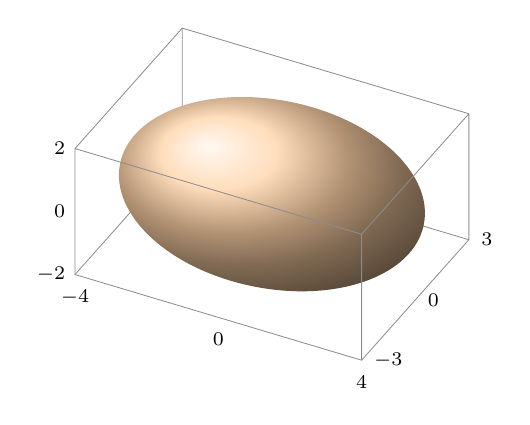
\begin{tikzpicture}[x={(0.455cm,-0.136cm)},y={(0.227cm,0.255cm)},z={(0cm,0.4cm)},
    font=\scriptsize,edge/.style={black!45,line width=.3pt}]
  \draw[edge] (4,3,-2)--(-4,3,-2)--(-4,-3,-2) (-4,3,-2)--(-4,3,2);
  \shade[ball color=orange!35!white,rotate=-11.3] (0,0) ellipse
    [x radius=1.967cm,y radius=1.195cm];
  \draw[edge] (-4,-3,-2)--(4,-3,-2)--(4,3,-2)--(4,3,2)--(-4,3,2)--(-4,-3,2)--cycle
    (4,-3,-2)--(4,-3,2)--(4,3,2) (4,-3,2)--(-4,-3,2);
  \foreach \z in {-2,0,2} \node[left] at (-4,-3,\z) {$\z$};
  \foreach \x in {-4,0,4} \node[below=2pt] at (\x,-3,-2) {$\x$};
  \foreach \y in {-3,0,3} \node[right=1pt] at (4,\y,-2) {$\y$};
\end{tikzpicture}
\end{minipage}\hfill
\begin{minipage}[c]{.36\linewidth}\centering
\captionof*{figure}{The ellipsoid $E(4f_1,3f_2,2f_3)$ in $\R^3$, where
$f_1,f_2,f_3$ is the standard basis of $\R^3$.}
\end{minipage}
\end{center}
\end{example}

The ellipsoid $E(f_1,\dots,f_n)$ equals the ball $B$ in $V$ for every
orthonormal basis $f_1,\dots,f_n$ of $V$ [by Parseval's identity
\ref{ax:6.30}(b)].

\begin{notation}[$T(\Omega)$]\label{ax:7.98}
For $T$ a function defined on $V$ and $\Omega\subseteq V$, define $T(\Omega)$
by
\[ T(\Omega) = \{Tv : v\in\Omega\}. \]
\end{notation}

Thus if $T$ is a function defined on $V$, then $T(V)=\range T$.

The next result states that every invertible operator $T\in\Lin(V)$ maps the
ball $B$ in $V$ onto an ellipsoid in $V$. The proof shows that the principal
axes of this ellipsoid come from the singular value decomposition of $T$.

\begin{result}[Invertible operator takes ball to ellipsoid]\label{ax:7.99}
Suppose $T\in\Lin(V)$ is invertible. Then $T$ maps the ball $B$ in $V$ onto an
ellipsoid in $V$.
\end{result}

\begin{proof}
Suppose $T$ has singular value decomposition
\[ Tv = s_1\ip{v}{e_1}f_1+\cdots+s_n\ip{v}{e_n}f_n \axeqno\label{ax:7.100} \]
for all $v\in V$; here $s_1,\dots,s_n$ are the singular values of $T$ and
$e_1,\dots,e_n$ and $f_1,\dots,f_n$ are both orthonormal bases of $V$. We will
show that $T(B)=E(s_1f_1,\dots,s_nf_n)$.

First suppose $v\in B$. Because $T$ is invertible, none of the singular values
$s_1,\dots,s_n$ equals $0$ (see \ref{ax:7.68}). Thus \ref{ax:7.100} implies
that
\[ \frac{\abs{\ip{Tv}{f_1}}^2}{s_1^2}+\cdots+\frac{\abs{\ip{Tv}{f_n}}^2}{s_n^2}
   = \abs{\ip{v}{e_1}}^2+\cdots+\abs{\ip{v}{e_n}}^2 < 1. \]
Thus $Tv\in E(s_1f_1,\dots,s_nf_n)$. Hence $T(B)\subseteq
E(s_1f_1,\dots,s_nf_n)$.

To prove inclusion in the other direction, now suppose
$w\in E(s_1f_1,\dots,s_nf_n)$. Let
\[ v = \frac{\ip{w}{f_1}}{s_1}e_1+\cdots+\frac{\ip{w}{f_n}}{s_n}e_n. \]
Then $\norm{v}<1$ and \ref{ax:7.100} implies that
$Tv=\ip{w}{f_1}f_1+\cdots+\ip{w}{f_n}f_n=w$. Thus
$T(B)\supseteq E(s_1f_1,\dots,s_nf_n)$.
\end{proof}

We now use the previous result to show that invertible operators take all
ellipsoids, not just the ball of radius $1$, to ellipsoids.

\begin{result}[Invertible operator takes ellipsoids to ellipsoids]\label{ax:7.101}
Suppose $T\in\Lin(V)$ is invertible and $E$ is an ellipsoid in $V$. Then
$T(E)$ is an ellipsoid in $V$.
\end{result}

\begin{proof}
There exist an orthonormal basis $f_1,\dots,f_n$ of $V$ and positive numbers
$s_1,\dots,s_n$ such that $E=E(s_1f_1,\dots,s_nf_n)$. Define $S\in\Lin(V)$ by
\[ S(a_1f_1+\cdots+a_nf_n) = a_1s_1f_1+\cdots+a_ns_nf_n. \]
Then $S$ maps the ball $B$ of $V$ onto $E$, as you can verify. Thus
\[ T(E) = T\bigl(S(B)\bigr) = (TS)(B). \]
The equation above and \ref{ax:7.99}, applied to $TS$, show that $T(E)$ is an
ellipsoid in $V$.
\end{proof}

Recall (see \ref{ax:3.95}) that if $u\in V$ and $\Omega\subseteq V$ then
$u+\Omega$ is defined by
\[ u+\Omega = \{u+w : w\in\Omega\}. \]
Geometrically, the sets $\Omega$ and $u+\Omega$ look the same, but they are in
different locations.

In the following definition, if $\dim V=2$ then the word
\emph{parallelogram} is often used instead of \emph{parallelepiped}.

\begin{definition}[$P(v_1,\dots,v_n)$, parallelepiped]\label{ax:7.102}
Suppose $v_1,\dots,v_n$ is a basis of $V$. Let
\[ P(v_1,\dots,v_n) = \{a_1v_1+\cdots+a_nv_n : a_1,\dots,a_n\in(0,1)\}. \]
A \emph{parallelepiped} is a set of the form $u+P(v_1,\dots,v_n)$ for some
$u\in V$. The vectors $v_1,\dots,v_n$ are called the \emph{edges} of this
parallelepiped.
\end{definition}

\begin{example}[Parallelepipeds]\label{ax:7.103}\leavevmode
\begin{center}
\begin{minipage}[b]{.48\linewidth}\centering
\begin{tikzpicture}[xscale=1.3,yscale=1.3]
  \fill[axfigblue] (.3,.5)--(1.3,.5)--(2.3,1.5)--(1.3,1.5)--cycle;
  \draw[line width=.4pt] (-.15,0)--(2.45,0); \draw[line width=.4pt] (-.15,0)--(-.15,1.6);
  \foreach \t in {0.3,1.3,2.3}
    \draw (\t,0)--(\t,-.06) node[below,font=\scriptsize] {$\t$};
  \foreach \t in {0.5,1.5}
    \draw (-.15,\t)--(-.21,\t) node[left,font=\scriptsize] {$\t$};
  \draw[vec] (.3,.5)--node[below,font=\scriptsize]{$v_1$} (1.3,.5);
  \draw[vec] (.3,.5)--node[above left=-1pt,font=\scriptsize]{$v_2$} (1.3,1.5);
\end{tikzpicture}
\captionof*{figure}{The parallelepiped $(0.3,0.5)+P\bigl((1,0),(1,1)\bigr)$
in $\R^2$.}
\end{minipage}\hfill
\begin{minipage}[b]{.48\linewidth}\centering
\begin{tikzpicture}[scale=1.25]
  \coordinate (O) at (0,0); \coordinate (a) at (1,-.25);
  \coordinate (b) at (2.1,.15); \coordinate (c) at (.35,1.15);
  \fill[orange!12,opacity=.8] (O)--(b)--($(b)+(c)$)--(c)--cycle;
  \fill[orange!12,opacity=.8] (O)--(a)--($(a)+(c)$)--(c)--cycle;
  \fill[orange!8,opacity=.8] (c)--($(a)+(c)$)--($(a)+(b)+(c)$)--($(b)+(c)$)--cycle;
  \fill[orange!10,opacity=.8] (a)--($(a)+(b)$)--($(a)+(b)+(c)$)--($(a)+(c)$)--cycle;
  \draw[black!35,line width=.3pt] (a)--($(a)+(b)$)--(b) (c)--($(a)+(c)$)
    --($(a)+(b)+(c)$)--($(b)+(c)$)--cycle ($(a)+(c)$)--(a)
    ($(a)+(b)$)--($(a)+(b)+(c)$) (b)--($(b)+(c)$);
  \draw[vec] (O)--node[below,font=\scriptsize]{$v_1$} (a);
  \draw[vec] (O)--node[above,pos=.6,font=\scriptsize]{$v_2$} (b);
  \draw[vec] (O)--node[left,font=\scriptsize]{$v_3$} (c);
\end{tikzpicture}
\captionof*{figure}{A parallelepiped in $\R^3$.}
\end{minipage}
\end{center}
\end{example}

\begin{result}[Invertible operator takes parallelepipeds to
parallelepipeds]\label{ax:7.104}
Suppose $u\in V$, $v_1,\dots,\allowbreak v_n$ is a basis of $V$, and
$T\in\Lin(V)$ is invertible. Then
\[ T\bigl(u+P(v_1,\dots,v_n)\bigr) = Tu+P(Tv_1,\dots,Tv_n). \]
\end{result}

\begin{proof}
Because $T$ is invertible, the list $Tv_1,\dots,Tv_n$ is a basis of $V$. The
linearity of $T$ implies that
\[ T(u+a_1v_1+\cdots+a_nv_n) = Tu+a_1Tv_1+\cdots+a_nTv_n \]
for all $a_1,\dots,a_n\in(0,1)$. Thus
$T\bigl(u+P(v_1,\dots,v_n)\bigr)=Tu+P(Tv_1,\dots,Tv_n)$.
\end{proof}

Just as the rectangles are distinguished among the parallelograms in $\R^2$, we
give a special name to the parallelepipeds in $V$ whose defining edges are
orthogonal to each other.

\begin{definition}[Box]\label{ax:7.105}
A \emph{box} in $V$ is a set of the form
\[ u+P(r_1e_1,\dots,r_ne_n), \]
where $u\in V$ and $r_1,\dots,r_n$ are positive numbers and $e_1,\dots,e_n$ is
an orthonormal basis of $V$.
\end{definition}

Note that in the special case of $\R^2$ each box is a rectangle, but the
terminology \emph{box} can be used in all dimensions.

\begin{example}[Boxes]\label{ax:7.106}\leavevmode
\begin{center}
\begin{minipage}[b]{.48\linewidth}\centering
\begin{tikzpicture}[scale=1]
  \fill[axfigblue] (1,0)--(2,1)--(1,2)--(0,1)--cycle;
  \draw[line width=.4pt] (-.05,-.1)--(2.15,-.1); \draw[line width=.4pt] (-.05,-.1)--(-.05,2.1);
  \foreach \t in {1,2} {
    \draw (\t,-.1)--(\t,-.16) node[below,font=\scriptsize] {$\t$};
    \draw (-.05,\t)--(-.11,\t) node[left,font=\scriptsize] {$\t$};}
  \draw[vec] (1,0)--node[below right=-1pt,pos=.5,font=\scriptsize]{$\sqrt2 e_1$} (2,1);
  \draw[vec] (1,0)--node[below left=-1pt,pos=.5,font=\scriptsize]{$\sqrt2 e_2$} (0,1);
\end{tikzpicture}
\captionof*{figure}{The box $(1,0)+P(\sqrt2e_1,\sqrt2e_2)$, where
$e_1=\bigl(1/\sqrt2,1/\sqrt2\bigr)$ and
$e_2=\bigl(-1/\sqrt2,1/\sqrt2\bigr)$.}
\end{minipage}\hfill
\begin{minipage}[b]{.48\linewidth}\centering
\begin{tikzpicture}[x={(1cm,-.33cm)},y={(.55cm,.55cm)},z={(0cm,.95cm)}]
  \fill[blue!8,opacity=.8] (0,0,0)--(0,2,0)--(0,2,1)--(0,0,1)--cycle;
  \fill[red!8,opacity=.8] (0,0,0)--(1,0,0)--(1,0,1)--(0,0,1)--cycle;
  \fill[orange!10,opacity=.8] (0,0,1)--(1,0,1)--(1,2,1)--(0,2,1)--cycle;
  \fill[black!5,opacity=.8] (1,0,0)--(1,2,0)--(1,2,1)--(1,0,1)--cycle;
  \draw[black!35,line width=.3pt] (1,0,0)--(1,2,0)--(0,2,0) (0,0,1)--(1,0,1)
    --(1,2,1)--(0,2,1)--cycle (1,0,0)--(1,0,1) (1,2,0)--(1,2,1) (0,2,0)--(0,2,1);
  \draw[vec] (0,0,0)--node[below,font=\scriptsize]{$e_1$} (1,0,0);
  \draw[vec] (0,0,0)--node[above left=-1pt,pos=.7,font=\scriptsize]{$2e_2$} (0,2,0);
  \draw[vec] (0,0,0)--node[left,font=\scriptsize]{$e_3$} (0,0,1);
\end{tikzpicture}
\captionof*{figure}{The box $P(e_1,2e_2,e_3)$, where $e_1,e_2,e_3$ is the
standard basis of $\R^3$.}
\end{minipage}
\end{center}
\end{example}

Suppose $T\in\Lin(V)$ is invertible. Then $T$ maps every parallelepiped in $V$
to a parallelepiped in $V$ (by \ref{ax:7.104}). In particular, $T$ maps every
box in $V$ to a parallelepiped in $V$. This raises the question of whether $T$
maps some boxes in $V$ to boxes in $V$. The following result answers this
question, with the help of the singular value decomposition.

\begin{result}[Every invertible operator takes some boxes to boxes]\label{ax:7.107}
Suppose $T\in\Lin(V)$ is invertible. Suppose $T$ has singular value
decomposition
\[ Tv = s_1\ip{v}{e_1}f_1+\cdots+s_n\ip{v}{e_n}f_n, \]
where $s_1,\dots,s_n$ are the singular values of $T$ and $e_1,\dots,e_n$ and
$f_1,\dots,f_n$ are orthonormal bases of $V$ and the equation above holds for
all $v\in V$. Then $T$ maps the box $u+P(r_1e_1,\dots,r_ne_n)$ onto the box
$Tu+P(r_1s_1f_1,\dots,r_ns_nf_n)$ for all positive numbers $r_1,\dots,r_n$ and
all $u\in V$.
\end{result}

\begin{proof}
If $a_1,\dots,a_n\in(0,1)$ and $r_1,\dots,r_n$ are positive numbers and
$u\in V$, then
\[ T(u+a_1r_1e_1+\cdots+a_nr_ne_n) = Tu+a_1r_1s_1f_1+\cdots+a_nr_ns_nf_n. \]
Thus $T\bigl(u+P(r_1e_1,\dots,r_ne_n)\bigr)=Tu+P(r_1s_1f_1,\dots,r_ns_nf_n)$.
\end{proof}

\subsection{Volume via Singular Values}

Our goal in this subsection is to understand how an operator changes the volume
of subsets of its domain. Because notions of volume belong to analysis rather
than to linear algebra, we will work only with an intuitive notion of volume.
Our intuitive approach to volume can be converted into appropriate correct
definitions, correct statements, and correct proofs using the machinery of
analysis.

Our intuition about volume works best in real inner product spaces. Thus the
assumption that $\F=\R$ will appear frequently in the rest of this subsection.

If $\dim V=n$, then by \emph{volume} we will mean $n$-dimensional volume. You
should be familiar with this concept in $\R^3$. When $n=2$, this is usually
called area instead of volume, but for consistency we use the word volume in
all dimensions. The most fundamental intuition about volume is that the volume
of a box (whose defining edges are by definition orthogonal to each other) is
the product of the lengths of the defining edges. Thus we make the following
definition.

\begin{definition}[Volume of a box]\label{ax:7.108}
Suppose $\F=\R$. If $u\in V$ and $r_1,\dots,r_n$ are positive numbers and
$e_1,\dots,e_n$ is an orthonormal basis of $V$, then
\[ \operatorname{volume}\bigl(u+P(r_1e_1,\dots,r_ne_n)\bigr)
   = r_1\times\cdots\times r_n. \]
\end{definition}

The definition above agrees with the familiar formulas for the area (which we
are calling the volume) of a rectangle in $\R^2$ and for the volume of a box in
$\R^3$. For example, the first box in Example~\ref{ax:7.106} has
two-dimensional volume (or area) $2$ because the defining edges of that box
have length $\sqrt2$ and $\sqrt2$. The second box in Example~\ref{ax:7.106}
has three-dimensional volume $2$ because the defining edges of that box have
length $1$, $2$, and $1$.

\marginfig{\begin{tikzpicture}[scale=.75]
  \fill[axfigblue] (0,0) circle (1);
  \draw[line width=.4pt] (-.68,-.68) rectangle (.68,.68)
    (.68,-.55) rectangle (.97,.55) (-.68,-.55) rectangle (-.97,.55)
    (-.55,.68) rectangle (.55,.97) (-.55,-.68) rectangle (.55,-.97);
\end{tikzpicture}}{Volume of this ball $\approx$ sum of the volumes of the five
boxes.}%
To define the volume of a subset of $V$, approximate the subset by a finite
collection of disjoint boxes, and then add up the volumes of the approximating
collection of boxes. As we approximate a subset of $V$ more accurately by
disjoint unions of more boxes, we get a better approximation to the volume.

These ideas should remind you of how the Riemann integral is defined by
approximating the area under a curve by a disjoint collection of rectangles.
This discussion leads to the following nonrigorous but intuitive definition.

\begin{definition}[Volume]\label{ax:7.109}
Suppose $\F=\R$ and $\Omega\subseteq V$. Then the \emph{volume} of $\Omega$,
denoted by $\operatorname{volume}\Omega$, is approximately the sum of the
volumes of a collection of disjoint boxes that approximate $\Omega$.
\end{definition}

\marginfig{\begin{tikzpicture}[xscale=1.5,yscale=.75]
  \fill[axfigblue] (0,0) circle (1);
  \draw[line width=.4pt] (-.68,-.68) rectangle (.68,.68)
    (.68,-.55) rectangle (.97,.55) (-.68,-.55) rectangle (-.97,.55)
    (-.55,.68) rectangle (.55,.97) (-.55,-.68) rectangle (.55,-.97);
\end{tikzpicture}}{Each box here has twice the width and the same height as
the boxes in the previous figure.}%
We are ignoring many reasonable questions by taking an intuitive approach to
volume. For example, if we approximate $\Omega$ by boxes with respect to one
basis, do we get the same volume if we approximate $\Omega$ by boxes with
respect to a different basis? If $\Omega_1$ and $\Omega_2$ are disjoint
subsets of $V$, is
$\operatorname{volume}(\Omega_1\cup\Omega_2)
=\operatorname{volume}\Omega_1+\operatorname{volume}\Omega_2$? Provided that
we consider only reasonably nice subsets of $V$, techniques of analysis show
that both these questions have affirmative answers that agree with our
intuition about volume.

\begin{example}[Volume change by a linear map]\label{ax:7.110}
Suppose that $T\in\Lin(\R^2)$ is defined by
$Tv=\allowbreak2\ip{v}{e_1}e_1+\ip{v}{e_2}e_2$, where $e_1,e_2$ is the standard basis of
$\R^2$. This linear map stretches vectors along the $e_1$-axis by a factor of
$2$ and leaves vectors along the $e_2$-axis unchanged. The ball approximated by
five boxes above gets mapped by $T$ to the ellipsoid shown here. Each of the
five boxes in the original figure gets mapped to a box of twice the width and
the same height as in the original figure. Hence each box gets mapped to a box
of twice the volume (area) as in the original figure. The sum of the volumes of
the five new boxes approximates the volume of the ellipsoid. Thus $T$ changes
the volume of the ball by a factor of $2$.
\end{example}

In the example above, $T$ maps boxes with respect to the basis $e_1,e_2$ to
boxes with respect to the same basis; thus we can see how $T$ changes volume.
In general, an operator maps boxes to parallelepipeds that are not boxes.
However, if we choose the right basis (coming from the singular value
decomposition!), then boxes with respect to that basis get mapped to boxes
with respect to a possibly different basis, as shown in \ref{ax:7.107}. This
observation leads to a natural proof of the following result.

\begin{result}[Volume changes by a factor of the product of the singular
values]\label{ax:7.111}
Suppose $\F=\R$, $T\in\Lin(V)$ is invertible, and $\Omega\subseteq V$. Then
\[ \operatorname{volume}T(\Omega)
   = (\text{product of singular values of }T)(\operatorname{volume}\Omega). \]
\end{result}

\begin{proof}
Suppose $T$ has singular value decomposition
\[ Tv = s_1\ip{v}{e_1}f_1+\cdots+s_n\ip{v}{e_n}f_n \]
for all $v\in V$, where $e_1,\dots,e_n$ and $f_1,\dots,f_n$ are orthonormal
bases of $V$.

Approximate $\Omega$ by boxes of the form $u+P(r_1e_1,\dots,r_ne_n)$, which
have volume $r_1\times\cdots\times r_n$. The operator $T$ maps each box
$u+P(r_1e_1,\dots,r_ne_n)$ onto the box $Tu+P(r_1s_1f_1,\dots,r_ns_nf_n)$,
which has volume $(s_1\times\cdots\times s_n)(r_1\times\cdots\times r_n)$.

The operator $T$ maps a collection of boxes that approximate $\Omega$ onto a
collection of boxes that approximate $T(\Omega)$. Because $T$ changes the
volume of each box in a collection that approximates $\Omega$ by a factor of
$s_1\times\cdots\times s_n$, the linear map $T$ changes the volume of $\Omega$
by the same factor.
\end{proof}

Suppose $T\in\Lin(V)$. As we will see when we get to determinants, the product
of the singular values of $T$ equals $\abs{\det T}$; see \ref{ax:9.60} and
\ref{ax:9.61}.

\subsection{Properties of an Operator as Determined by Its Eigenvalues}

We conclude this chapter by presenting the table below. The context of this
table is a finite-dimensional complex inner product space. The first column of
the table shows a property that a normal operator on such a space might have.
The second column of the table shows a subset of $\C$ such that the operator
has the corresponding property if and only if all eigenvalues of the operator
lie in the specified subset. For example, the first row of the table states
that a normal operator is invertible if and only if all its eigenvalues are
nonzero (this first row is the only one in the table that does not need the
hypothesis that the operator is normal).

Make sure you can explain why all results in the table hold. For example, the
last row of the table holds because the norm of an operator equals its largest
singular value (by \ref{ax:7.85}) and the singular values of a normal
operator, assuming $\F=\C$, equal the absolute values of the eigenvalues (by
Exercise~7 in Section~7E).

\begin{center}\small
\begin{tabular}{l|l}
\multicolumn{1}{l}{\textbf{properties of a normal operator}} &
  \multicolumn{1}{l}{\textbf{eigenvalues are contained in}}\\
\hline
invertible & $\C\setminus\{0\}$\\ \hline
self-adjoint & $\R$\\ \hline
skew & $\{\lambda\in\C : \Re\lambda=0\}$\\ \hline
orthogonal projection & $\{0,1\}$\\ \hline
positive & $[0,\infty)$\\ \hline
unitary & $\{\lambda\in\C : \abs{\lambda}=1\}$\\ \hline
norm is less than $1$ & $\{\lambda\in\C : \abs{\lambda}<1\}$\\ \hline
\end{tabular}
\end{center}

% ------------------------------------------------------------------ exercises
\begin{exc}

\begin{exercise}
Prove that if $S,T\in\Lin(V,W)$, then
$\bigl\lvert\norm{S}-\norm{T}\bigr\rvert\le\norm{S-T}$.
\exnote{The inequality above is called the \textbf{reverse triangle
inequality}.}
\end{exercise}

\begin{exercise}
Suppose that $T\in\Lin(V)$ is self-adjoint or that $\F=\C$ and $T\in\Lin(V)$
is normal. Prove that
\[ \norm{T} = \max\{\abs{\lambda} : \lambda \text{ is an eigenvalue of } T\}. \]
\end{exercise}

\begin{exercise}
Suppose $T\in\Lin(V,W)$ and $v\in V$. Prove that
\[ \norm{Tv}=\norm{T}\,\norm{v} \iff T^*Tv=\norm{T}^2v. \]
\end{exercise}

\begin{exercise}
Suppose $T\in\Lin(V,W)$, $v\in V$, and $\norm{Tv}=\norm{T}\,\norm{v}$. Prove
that if $u\in V$ and $\ip{u}{v}=0$, then $\ip{Tu}{Tv}=0$.
\end{exercise}

\begin{exercise}
Suppose $U$ is a finite-dimensional inner product space, $T\in\Lin(V,U)$, and
$S\in\Lin(U,W)$. Prove that
\[ \norm{ST}\le\norm{S}\,\norm{T}. \]
\end{exercise}

\begin{exercise}
Prove or give a counterexample: If $S,T\in\Lin(V)$, then
$\norm{ST}=\norm{TS}$.
\end{exercise}

\begin{exercise}
Show that defining $d(S,T)=\norm{S-T}$ for $S,T\in\Lin(V,W)$ makes $d$ a
metric on $\Lin(V,W)$.
\exnote{This exercise is intended for readers who are familiar with metric
spaces.}
\end{exercise}

\begin{exercise}\leavevmode
\begin{parts}
\item Prove that if $T\in\Lin(V)$ and $\norm{I-T}<1$, then $T$ is invertible.
\item Suppose that $S\in\Lin(V)$ is invertible. Prove that if $T\in\Lin(V)$
  and $\norm{S-T}<1/\norm{S^{-1}}$, then $T$ is invertible.
\end{parts}
\exnote{This exercise shows that the set of invertible operators in $\Lin(V)$
is an open subset of $\Lin(V)$, using the metric defined in Exercise~7.}
\end{exercise}

\begin{exercise}
Suppose $T\in\Lin(V)$. Prove that for every $\epsilon>0$, there exists an
invertible operator $S\in\Lin(V)$ such that $0<\norm{T-S}<\epsilon$.
\end{exercise}

\begin{exercise}
Suppose $\dim V>1$ and $T\in\Lin(V)$ is not invertible. Prove that for every
$\epsilon>0$, there exists $S\in\Lin(V)$ such that $0<\norm{T-S}<\epsilon$ and
$S$ is not invertible.
\end{exercise}

\begin{exercise}
Suppose $\F=\C$ and $T\in\Lin(V)$. Prove that for every $\epsilon>0$ there
exists a diagonalizable operator $S\in\Lin(V)$ such that
$0<\norm{T-S}<\epsilon$.
\end{exercise}

\begin{exercise}
Suppose $T\in\Lin(V)$ is a positive operator. Show that
$\bigl\lVert\sqrt{T}\bigr\rVert=\sqrt{\norm{T}}$.
\end{exercise}

\begin{exercise}
Suppose $S,T\in\Lin(V)$ are positive operators. Show that
\[ \norm{S-T}\le\max\{\norm{S},\norm{T}\}\le\norm{S+T}. \]
\end{exercise}

\begin{exercise}
Suppose $U$ and $W$ are subspaces of $V$ such that $\norm{P_U-P_W}<1$. Prove
that $\dim U=\dim W$.
\end{exercise}

\begin{exercise}
Define $T\in\Lin(\F^3)$ by
\[ T(z_1,z_2,z_3) = (z_3,2z_1,3z_2). \]
Find (explicitly) a unitary operator $S\in\Lin(\F^3)$ such that
$T=S\sqrt{T^*T}$.
\end{exercise}

\begin{exercise}
Suppose $S\in\Lin(V)$ is a positive invertible operator. Prove that there
exists $\delta>0$ such that $T$ is a positive operator for every self-adjoint
operator $T\in\Lin(V)$ with $\norm{S-T}<\delta$.
\end{exercise}

\begin{exercise}
Prove that if $u\in V$ and $\varphi_u$ is the linear functional on $V$ defined
by the equation $\varphi_u(v)=\ip{v}{u}$, then $\norm{\varphi_u}=\norm{u}$.
\exnote{Here we are thinking of the scalar field $\F$ as an inner product
space with $\ip{\alpha}{\beta}=\alpha\overline{\beta}$ for all
$\alpha,\beta\in\F$. Thus $\norm{\varphi_u}$ means the norm of $\varphi_u$ as a
linear map from $V$ to $\F$.}
\end{exercise}

\begin{exercise}
Suppose $e_1,\dots,e_n$ is an orthonormal basis of $V$ and $T\in\Lin(V,W)$.
\begin{parts}
\item Prove that
  $\max\{\norm{Te_1},\dots,\norm{Te_n}\}\le\norm{T}
  \le(\norm{Te_1}^2+\cdots+\norm{Te_n}^2)^{1/2}$.
\item Prove that $\norm{T}=(\norm{Te_1}^2+\cdots+\norm{Te_n}^2)^{1/2}$
  if and only if $\dim\range T\le1$.
\end{parts}
\exnote{Here $e_1,\dots,e_n$ is an arbitrary orthonormal basis of $V$, not
necessarily connected with a singular value decomposition of $T$. If
$s_1,\dots,s_n$ is the list of singular values of $T$, then the right side of
the inequality above equals $(s_1^2+\cdots+s_n^2)^{1/2}$, as was shown in
Exercise~11(a) in Section~7E.}
\end{exercise}

\begin{exercise}
Prove that if $T\in\Lin(V,W)$, then $\norm{T^*T}=\norm{T}^2$.
\exnote{This formula for $\norm{T^*T}$ leads to the important subject of
$C^*$-algebras.}
\end{exercise}

\begin{exercise}
Suppose $T\in\Lin(V)$ is normal. Prove that $\norm{T^k}=\norm{T}^k$ for every
positive integer $k$.
\end{exercise}

\begin{exercise}
Suppose $\dim V>1$ and $\dim W>1$. Prove that the norm on $\Lin(V,W)$ does not
come from an inner product. In other words, prove that there does not exist an
inner product on $\Lin(V,W)$ such that
\[ \max\{\norm{Tv} : v\in V \text{ and } \norm{v}\le1\} = \sqrt{\ip{T}{T}} \]
for all $T\in\Lin(V,W)$.
\end{exercise}

\begin{exercise}
Suppose $T\in\Lin(V,W)$. Let $n=\dim V$ and let $s_1\ge\cdots\ge s_n$ denote
the singular values of $T$. Prove that if $1\le k\le n$, then
\[ \min\{\norm{T|_U} : U \text{ is a subspace of } V \text{ with }
   \dim U=k\} = s_{n-k+1}. \]
\end{exercise}

\begin{exercise}
Suppose $T\in\Lin(V,W)$. Show that $T$ is uniformly continuous with respect to
the metrics on $V$ and $W$ that arise from the norms on those spaces (see
Exercise~23 in Section~6B).
\end{exercise}

\begin{exercise}
Suppose $T\in\Lin(V)$ is invertible. Prove that
\[ \norm{T^{-1}}=\norm{T}^{-1} \iff \frac{T}{\norm{T}}
   \text{ is a unitary operator.} \]
\end{exercise}

\begin{exercise}
Fix $u,x\in V$ with $u\ne0$. Define $T\in\Lin(V)$ by $Tv=\ip{v}{u}x$ for every
$v\in V$. Prove that
\[ \sqrt{T^*T}\,v = \frac{\norm{x}}{\norm{u}}\ip{v}{u}u \]
for every $v\in V$.
\end{exercise}

\begin{exercise}
Suppose $T\in\Lin(V)$. Prove that $T$ is invertible if and only if there
exists a unique unitary operator $S\in\Lin(V)$ such that $T=S\sqrt{T^*T}$.
\end{exercise}

\begin{exercise}
Suppose $T\in\Lin(V)$ and $s_1,\dots,s_n$ are the singular values of $T$. Let
$e_1,\dots,e_n$ and $f_1,\dots,f_n$ be orthonormal bases of $V$ such that
\[ Tv = s_1\ip{v}{e_1}f_1+\cdots+s_n\ip{v}{e_n}f_n \]
for all $v\in V$. Define $S\in\Lin(V)$ by
\[ Sv = \ip{v}{e_1}f_1+\cdots+\ip{v}{e_n}f_n. \]
\begin{parts}
\item Show that $S$ is unitary and
  $\norm{T-S}=\max\{\abs{s_1-1},\dots,\abs{s_n-1}\}$.
\item Show that if $E\in\Lin(V)$ is unitary, then $\norm{T-E}\ge\norm{T-S}$.
\end{parts}
\exnote{This exercise finds a unitary operator $S$ that is as close as
possible (among the unitary operators) to a given operator $T$.}
\end{exercise}

\begin{exercise}
Suppose $T\in\Lin(V)$. Prove that there exists a unitary operator
$S\in\Lin(V)$ such that $T=\sqrt{TT^*}\,S$.
\end{exercise}

\begin{exercise}
Suppose $T\in\Lin(V)$.
\begin{parts}
\item Use the polar decomposition to show that there exists a unitary operator
  $S\in\Lin(V)$ such that $TT^*=ST^*TS^*$.
\item Show how (a) implies that $T$ and $T^*$ have the same singular values.
\end{parts}
\end{exercise}

\begin{exercise}
Suppose $T\in\Lin(V)$, $S\in\Lin(V)$ is a unitary operator, and $R\in\Lin(V)$
is a positive operator such that $T=SR$. Prove that $R=\sqrt{T^*T}$.
\exnote{This exercise shows that if we write $T$ as the product of a unitary
operator and a positive operator (as in the polar decomposition
\ref{ax:7.93}), then the positive operator equals $\sqrt{T^*T}$.}
\end{exercise}

\begin{exercise}
Suppose $\F=\C$ and $T\in\Lin(V)$ is normal. Prove that there exists a unitary
operator $S\in\Lin(V)$ such that $T=S\sqrt{T^*T}$ and such that $S$ and
$\sqrt{T^*T}$ both have diagonal matrices with respect to the same orthonormal
basis of $V$.
\end{exercise}

\begin{exercise}
Suppose that $T\in\Lin(V,W)$ and $T\ne0$. Let $s_1,\dots,s_m$ denote the
positive singular values of $T$. Show that there exists an orthonormal basis
$e_1,\dots,e_m$ of $(\nul T)^\perp$ such that
\[ T\Bigl(E\Bigl(\frac{e_1}{s_1},\dots,\frac{e_m}{s_m}\Bigr)\Bigr) \]
equals the ball in $\range T$ of radius $1$ centered at $0$.
\end{exercise}
\end{exc}
